\documentclass[12pt]{article}
\usepackage{amsmath}
\usepackage{epsfig}
\usepackage{lscape}
%\usepackage{rotating}
\usepackage{array}
\usepackage{natbib}
\usepackage{graphicx}
\usepackage{enumerate}
\topmargin 0in \headheight 0.0in \textheight 9in \textwidth 6.5in
\oddsidemargin 0.1in \evensidemargin 0.1in
\renewcommand{\baselinestretch}{1.3}
\newcommand{\beq}{\begin{equation}}
\newcommand{\eeq}{\end{equation}}
\newcommand{\ie}{\emph{i.e.}}
\newcommand{\eg}{\emph{e.g.}}



\graphicspath{{../Figures/}}






\begin{document}
\title{On connections between graph signal processing and eigenvector spatial filtering for analyzing biomedical imaging data}
\date{}
\maketitle

\section*{Comments and notes}

\begin{enumerate}[$\bullet$]
	\item \textbf{HAVING TROUBLE INCLUDING IMAGES?} This tex file is currently looking for figures by, relative to the directory containing the tex file, going up one directory and down into a Figures directory. This should correspond with the Figures directory of the ESFGSP\_Paper Github repo. Individual figure paths should thus be relative to the Figures directory. If the figure you're trying to include is in the Figures directory, this is just the figure file name.
	\item Note: Eigendecomposition, eigenvector, and eigenvalue are each one word.
	\item William comment: We want to be careful about hammering too much on imaging analysis as the typical application rather than our application of interest. It might be limiting to box ourselves in to `data obtained by taking some sort of picture/scan.'
	\begin{enumerate}
		\item It's not clear to me that the typical geostatistical usage is best classified as ``imaging analyses'' and we will rely heavily on geostatistical developments and methodologies in comparison. 
		\item GSP applications include literal network data such as data from social media platforms.
		\item Staying slightly less closely tied to images is also helpful for drawing comparisons, as geographical point data are irregularly located (point data) within a regular structure (space) while neuroimaging data are regularly located (voxel lattice) within an irregular structure (brain network), and it's the irregularity of each that really calls for network based approaches. 
	\end{enumerate}
	\item William comment: Regarding the lung eigenvector figure: 
	\begin{enumerate}
		\item I think we should drop EV300 and add in the constant eigenvector with eigenvalue 0. I think one of the advantages we want to highlight in the comparison of ESF and GSP is the utility of the centering matrix $\mathbf M$ for giving us notions of positive and negative correlation.
		\item I think making a corresponding figure using the same $\mathbf C$ but, say, a GSP Laplacian approach, would be informative. Maybe display the corresponding eigenvalues for the plots. I'm really hoping they look pretty similar, except maybe that ESF eigenvectors have zero constant component and GSP eigenvectors will have non-zero constant component.
		\item I think really focusing on visuals in the lung space will be an advantage for us in this paper. Unlike point data and neuroimaging data, this is regularly located data in a regular space. There is just a lot of stuff that's intuitive to consider in regular spatial contexts that are much harder to consider in irregularly structured contexts like brains.
	\end{enumerate}
	\item We may actually want to recreate some Moran formulas to really show the autocorrelation in summation notation more explicitly rather than pointing to a reference. I want someone familiar with GSP to look at ESF and the $\mathbf M$ business and say `Oh. That makes a lot of sense.'
\end{enumerate}


\section{Background}

This work is motivated by a desire to account for the complex spatial and biologic structure in analysis of biomedical imaging data (CT, neuroimaging, etc).

There have been two parallel developments in the literature - explain both and cite the literature.

Graph Signal Processing (GSP) comes from a generalization of theory behind the discrete Fourier transform or fast Fourier transform through generalization of the presumed underlying observation space, a discretized torus for classical Fourier theory, to a general network. In neuroimaging applications, estimation of (aspects of?) the network is one focus and extracting primary ``anatomically aligned'' signals for analysis (akin to largest PCs) is another. 

ESF is used to account for substantial spatial correlation in contexts where estimation of correlation structure directly from spatial data may not otherwise be feasible in order to improve inference on fixed non-spatial effects. For ESF, spatial structure can be reasonably well approximated through a priori specification of spatial covariance models and the structure itself is not of interest.

The purpose of this paper is to draw direct connections between these two parallel developments of [insert] and to apply various approaches from both areas to highlight the advantages and similarities of each approach to analyzing imaging data. We conduct analysis using a traditional ESF approach, prediction [outline more], and GSP approaches to estimate a network and use an estimated network to [do what]. We do this on a toy example to clearly exhibit the links between the approaches, on neuroimaging data in aging (BIOAD), and chest (lung) CT in sarcoidosis.

\section{Methods}

Both eigenvector spatial filtering (ESF) and graph signal processing (GSP) provide frameworks for representing inherent structure in an observation space, such as the spatial structure associated with data observed at various geographical locations or the network structure associated to the anatomy of the brain in neuroimaging. This representation is obtained through eigendecomposition of a matrix quantifying the structure of the observation space into eigenvectors representing various component patterns in observation space and eigenvalues that index and in some sense characterize the eigenvectors relative to the specified structure. 

ESF and GSP differ in how this matrix quantifying structure in observation space is specified and manipulated prior to eigendecomposition, resulting in differing properties of the resulting representation of the observation space. The fundamental theory and applications of interest associated with each also drives focus in methodological development utilizing these representations. We begin by defining the representations used.

\subsection{Defining representations}

\subsubsection{Eigenvector spatial filtering}
[Cut from Sarah Ryan paper so will need editing but will give you a notational start]. 

Eigenvector spatial filtering (ESF) is a technique used to efficiently account for spatial structure in spatially distributed data using linear combinations of spatial eigenvectors derived from a representation of the observation space \citep{griffith1996spatial}. The spatial eigenvectors are constructed by the eigendecomposition of a centered model spatial covariance matrix, such as from an exponential, gaussian, or spherical model. We note that the choice of spatial covariance matrix is typically made without reference to the observed data through specification of a spatial covariance model and parameters. As such, resulting eigenvectors are data independent. For the set of unique spatial locations, $S$, let $\mathbf{C}$ be an $(S \times S)$ symmetric spatial covariance matrix and $\mathbf{M}=I - 11^\prime/S$ be a centering matrix \citep{griffith1996spatial}. Then, $\mathbf{M} \mathbf{C} \mathbf{M}$ is eigendecomposed as $\mathbf{E}_\textit{full} \mathbf{\Lambda}_\textit{full} \mathbf{E}_\textit{full}'$, where $\mathbf{E}_\textit{full}$ is a orthogonal matrix comprised of spatial eigenvectors, called Moran eigenvectors, and $\mathbf{\Lambda}_\textit{full}$ is a diagonal matrix of eigenvalues proportional to a measure of spatial autocorrelation, Moran's $I$, with respect to weights $\mathbf{C}$; for more information regarding Moran, see \cite{murakami2019eigenvector} (also include a Moran reference).  

Centering the spatial structure $\mathbf C$ using $\mathbf M$ ensures that there is always a constant value Moran eigenvector associated with eigenvalue 0. In this way, eigenvectors with positive eigenvalues exhibit positive spatial autocorrelation and eigenvectors with negative eigenvalues exhibit negative spatial autocorrelation, with eigenvalue magnitude indicating degree of autocorrelation. The complete set of eigenvectors, $\mathbf{E}_\textit{full}$, provides an spatially orthogonal basis for all possible distinct patterns of spatial dependence for the given data structure or observation space relative to the specified spatial structure $\mathbf{C}$, where the first eigenvector has the largest spatial dependence and corresponds to the largest spatial structures; the second eigenvector has the second largest spatial dependence and corresponds to the second largest spatial pattern, and so forth; see Figure \ref{fig:eigenvectors} for visualizations of select eigenvectors in a template lung.

The resulting matrix $\mathbf{E}_{full}$ is then a representation of the observation space which is incorporated into ESF analyses.

The complete set of eigenvectors is not always considered necessary to adequately account for spatial patterns in the data. A subset of $L<<S$ eigenvectors corresponding with $(S\times L)$ submatrix $\mathbf{E}$ of $\mathbf{E}_{full}$ may be selected for use in analyses. Often, only eigenvectors associated with positive eigenvalues are selected, corresponding to positive spatial dependence, since positive spatial correlation is observed naturally \citep{griffith2014spatial, griffith2006spatial, chun2014quality}. 


\begin{figure}
\centering 
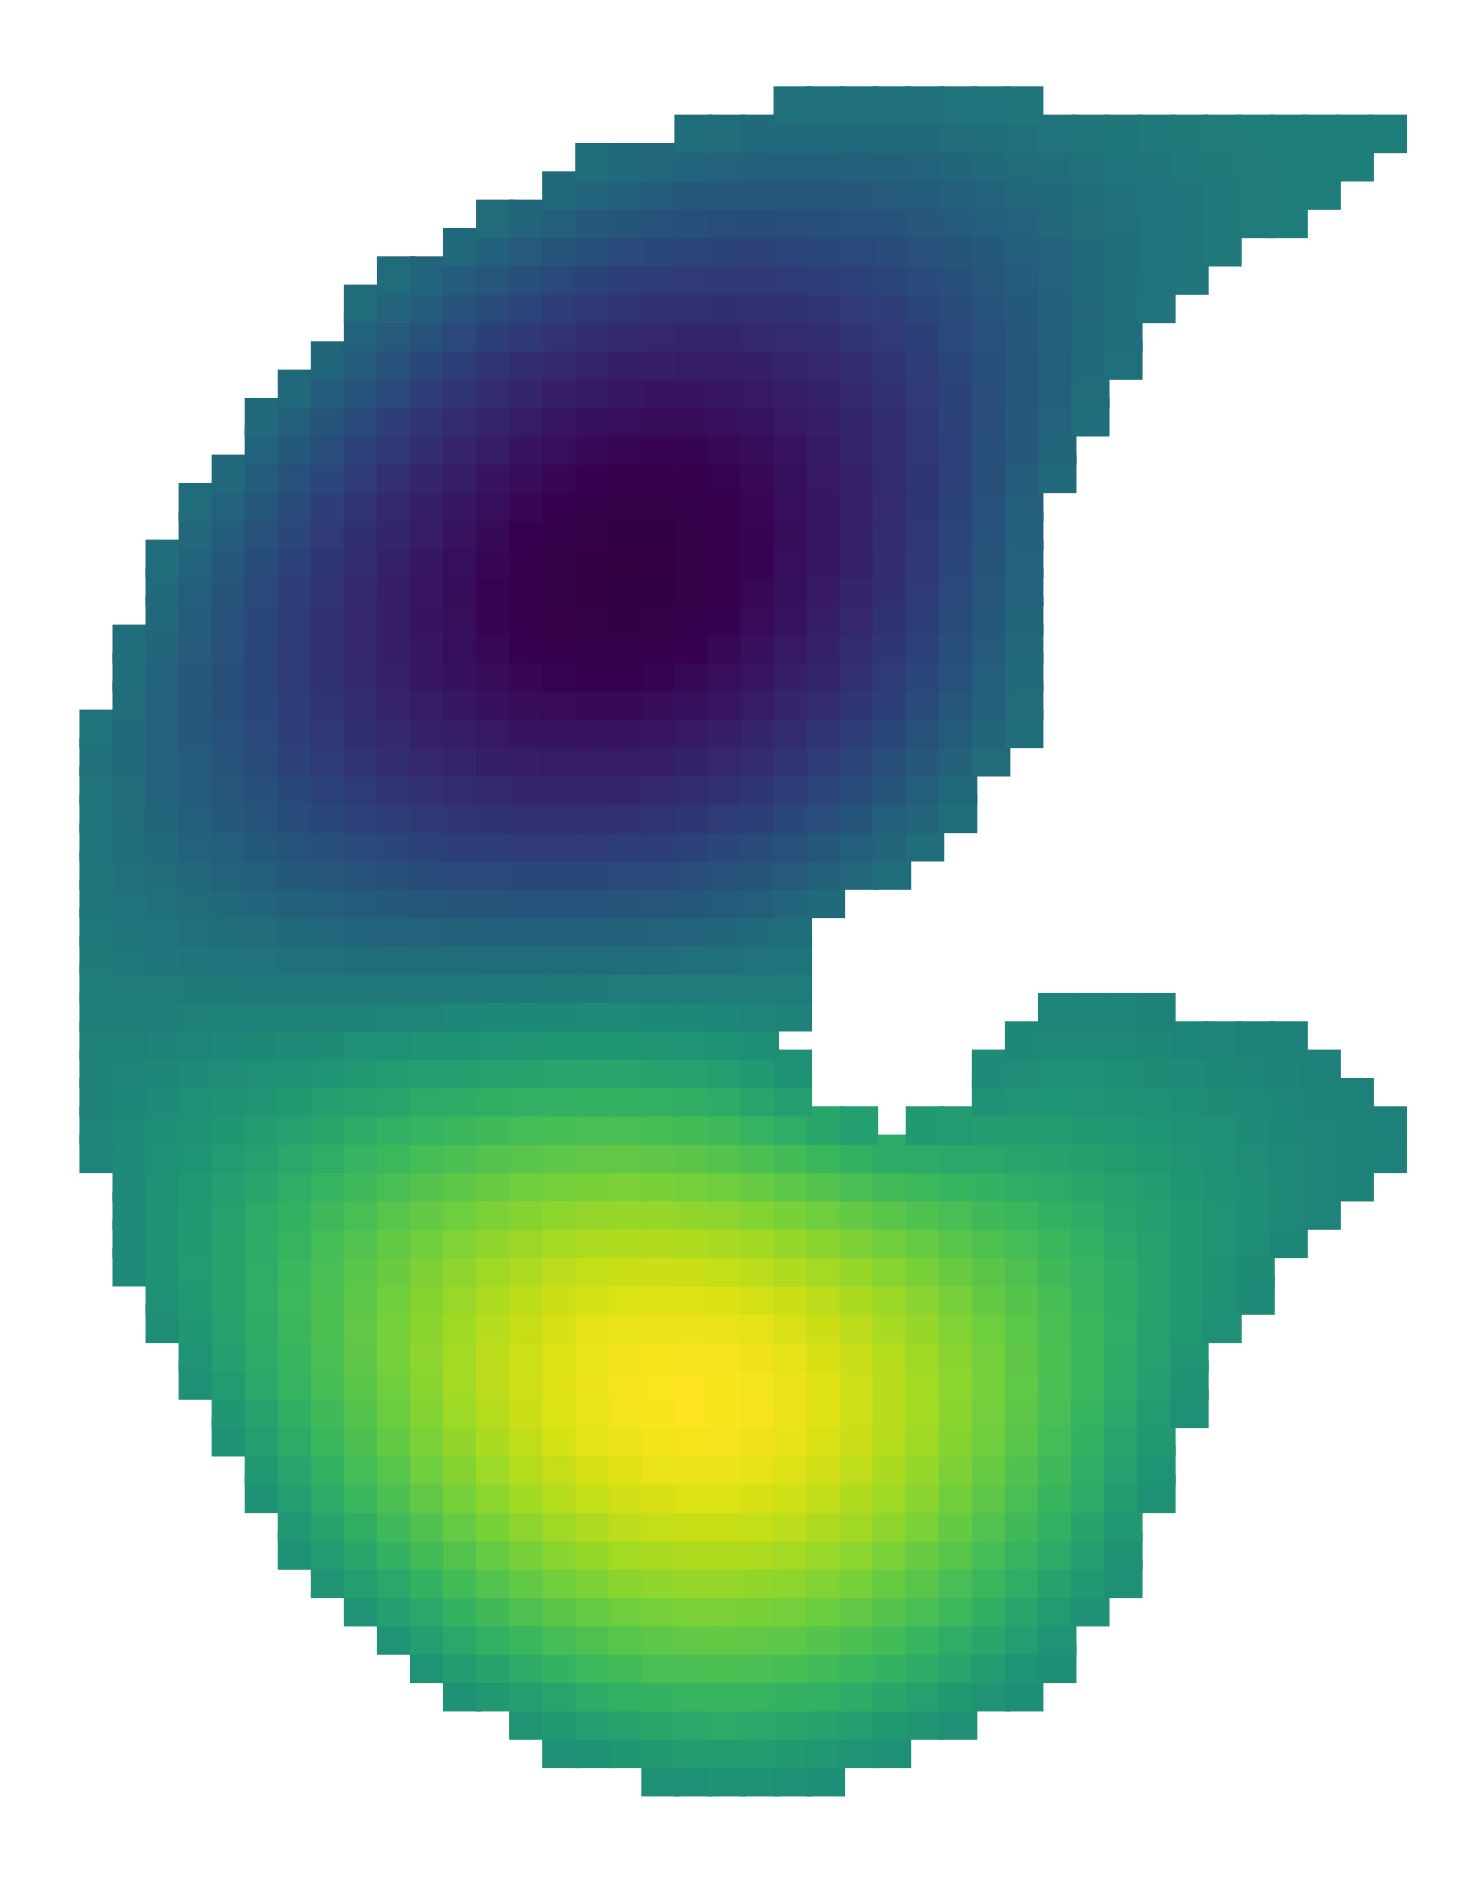
\includegraphics[height=1.5in]{EV1}
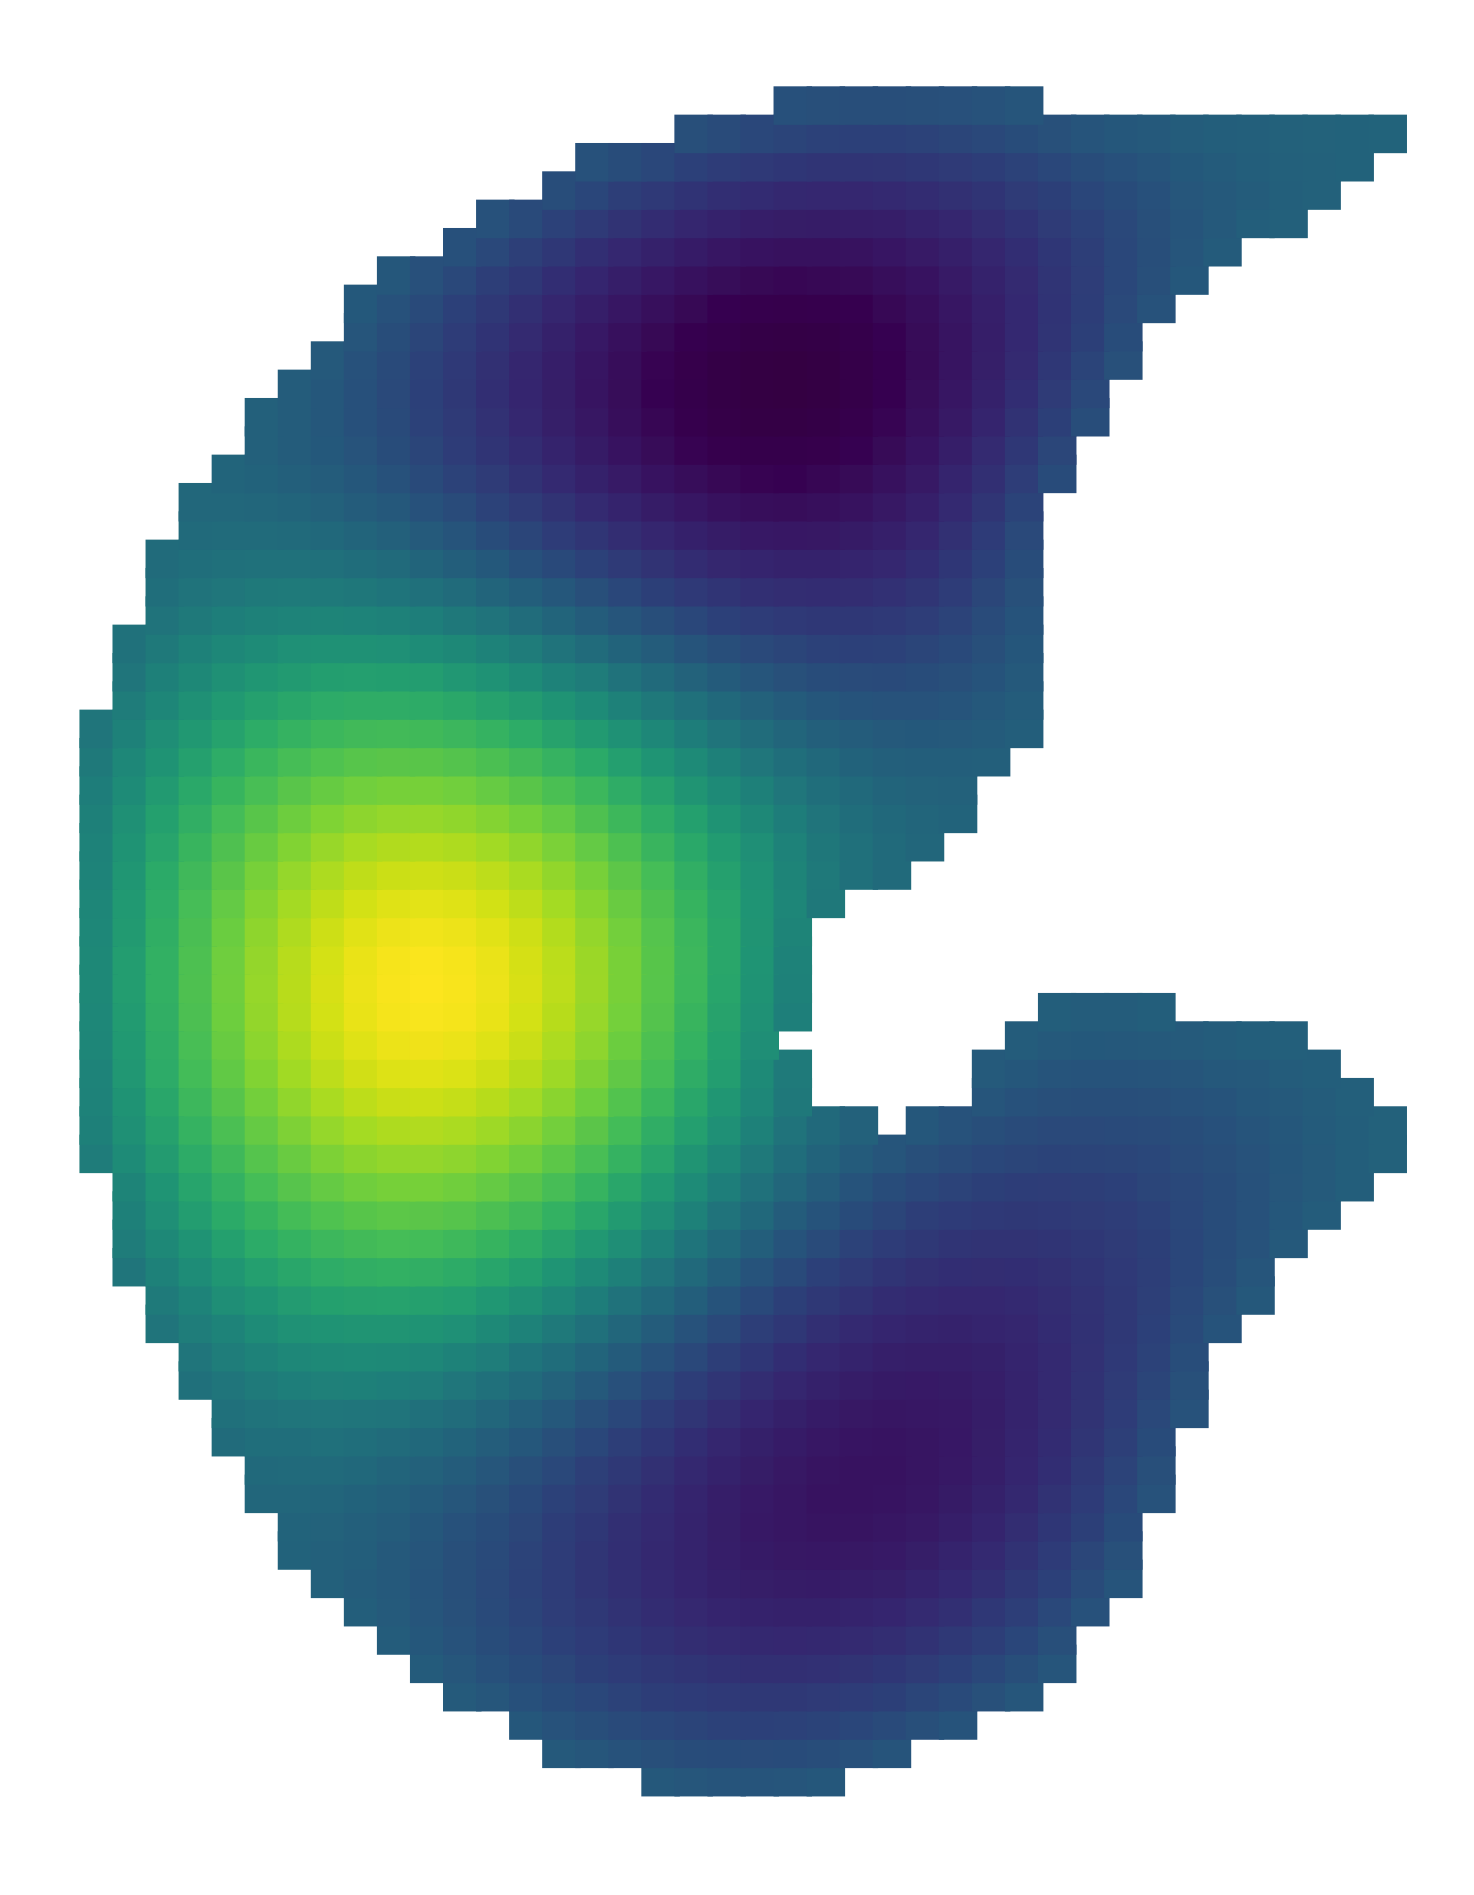
\includegraphics[height=1.5in]{EV2}
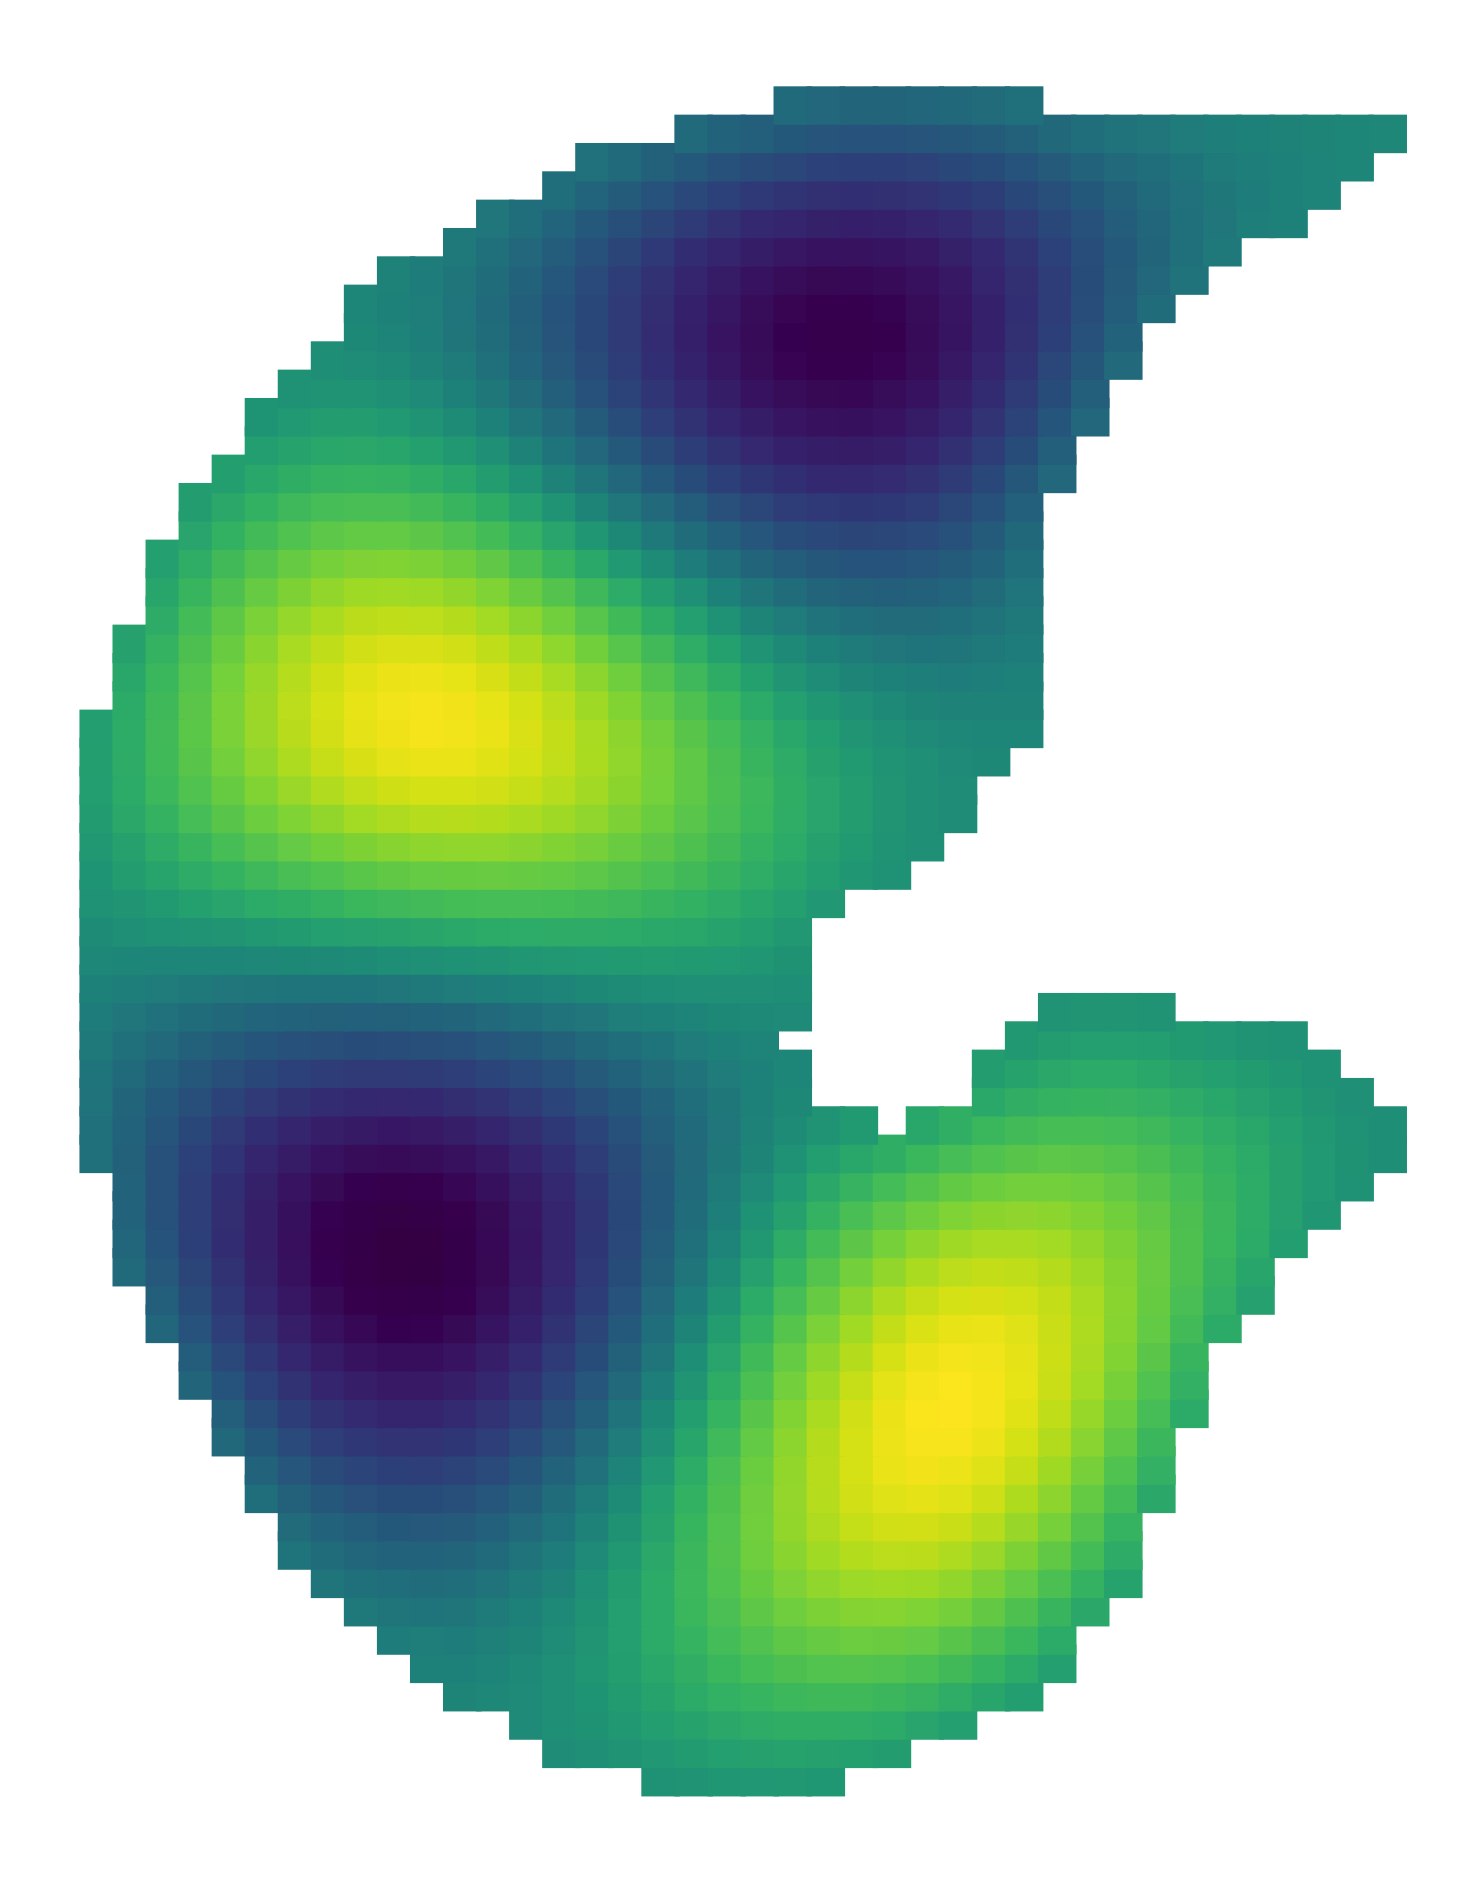
\includegraphics[height=1.5in]{EV3}
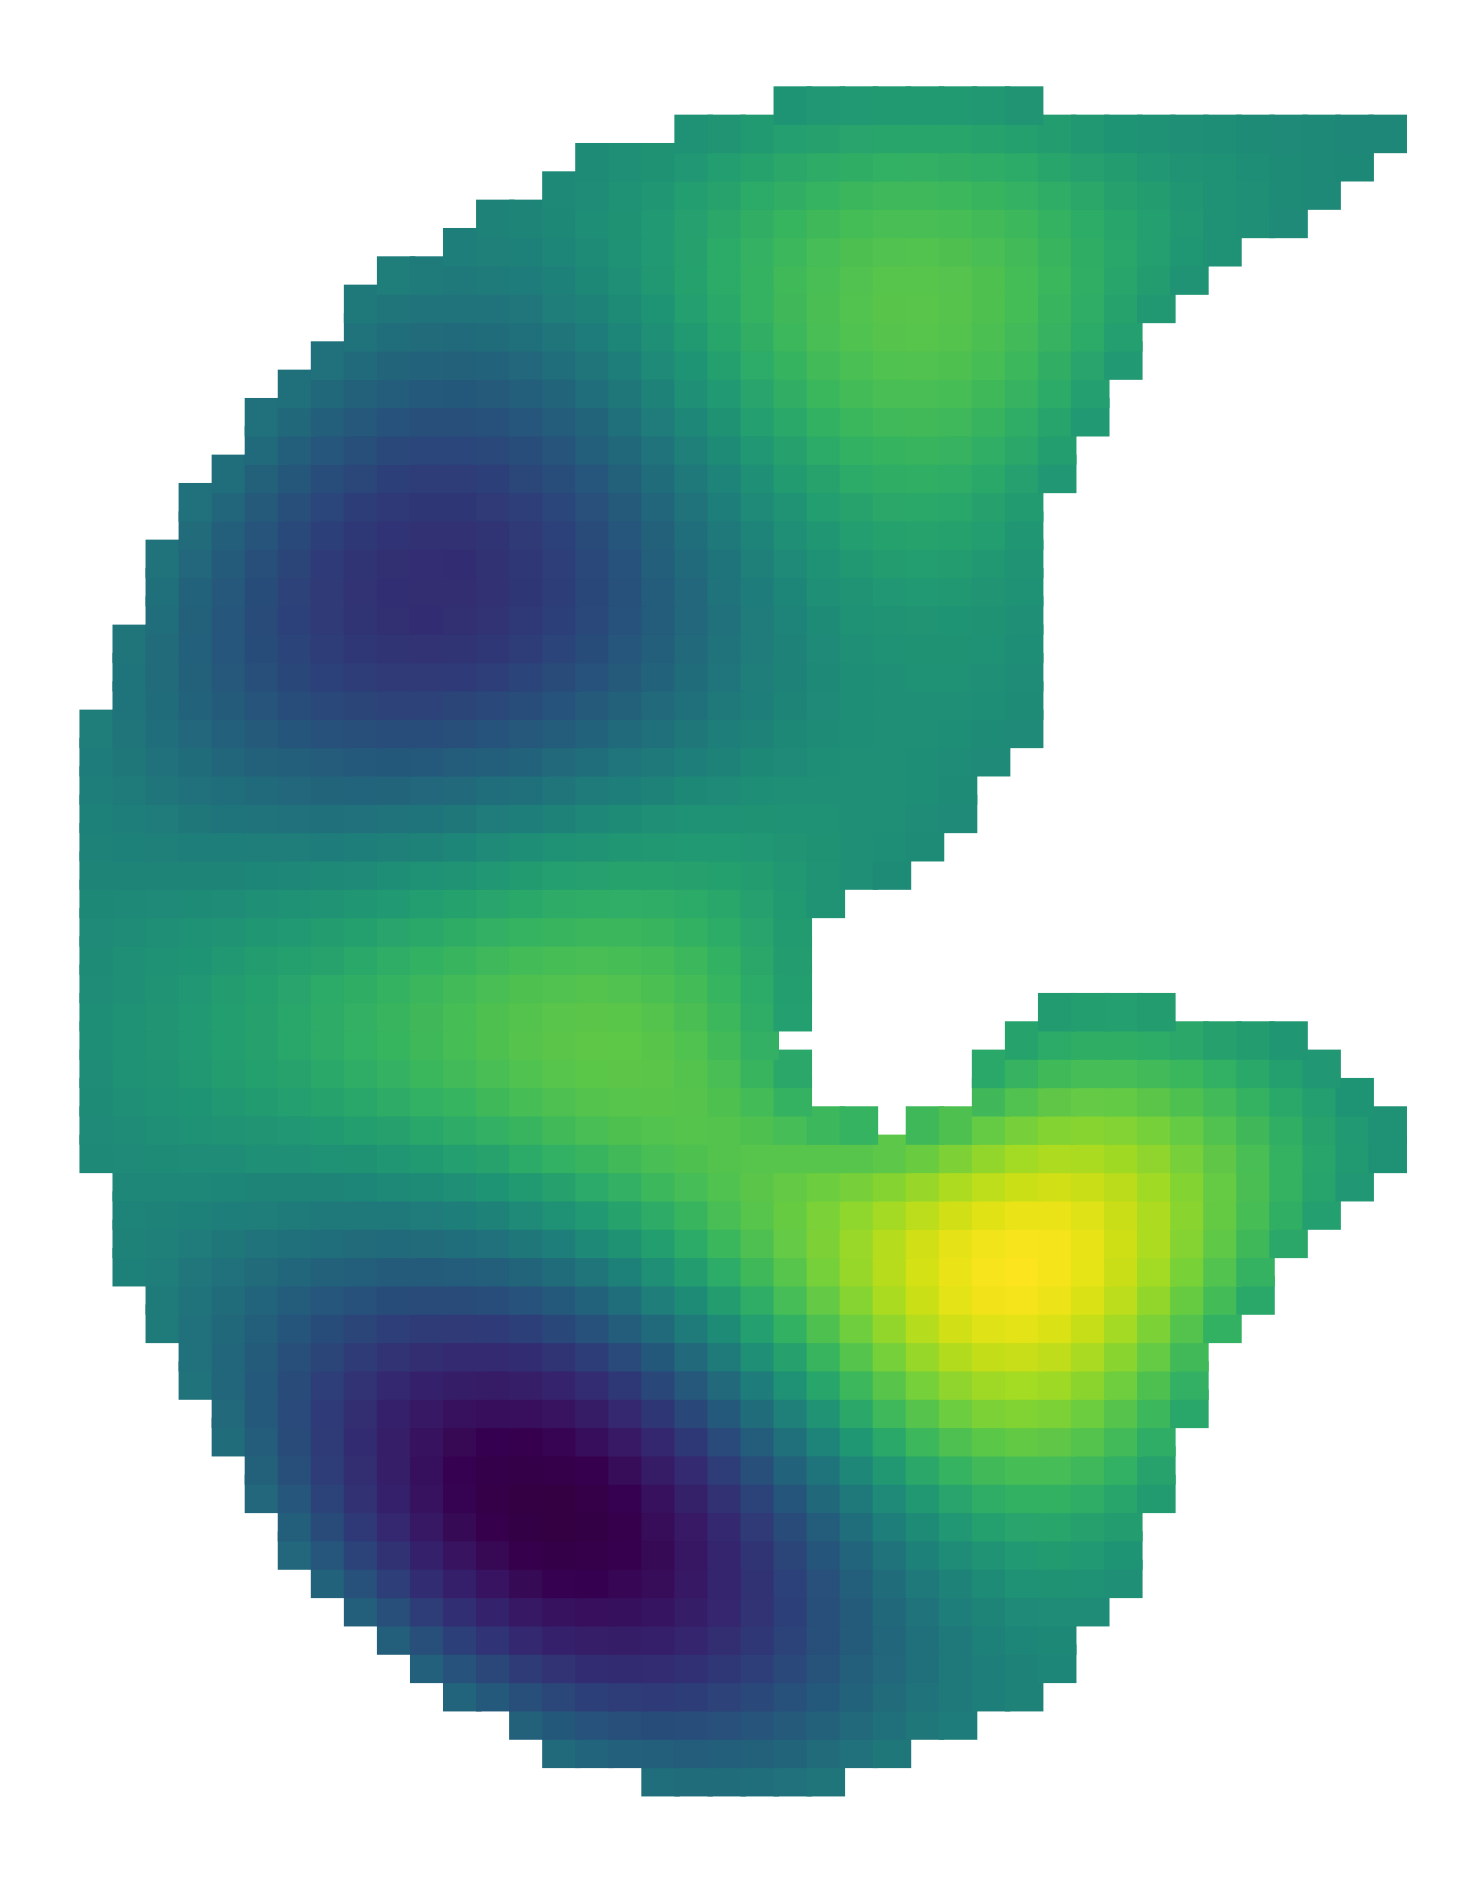
\includegraphics[height=1.5in]{EV4}\\ 

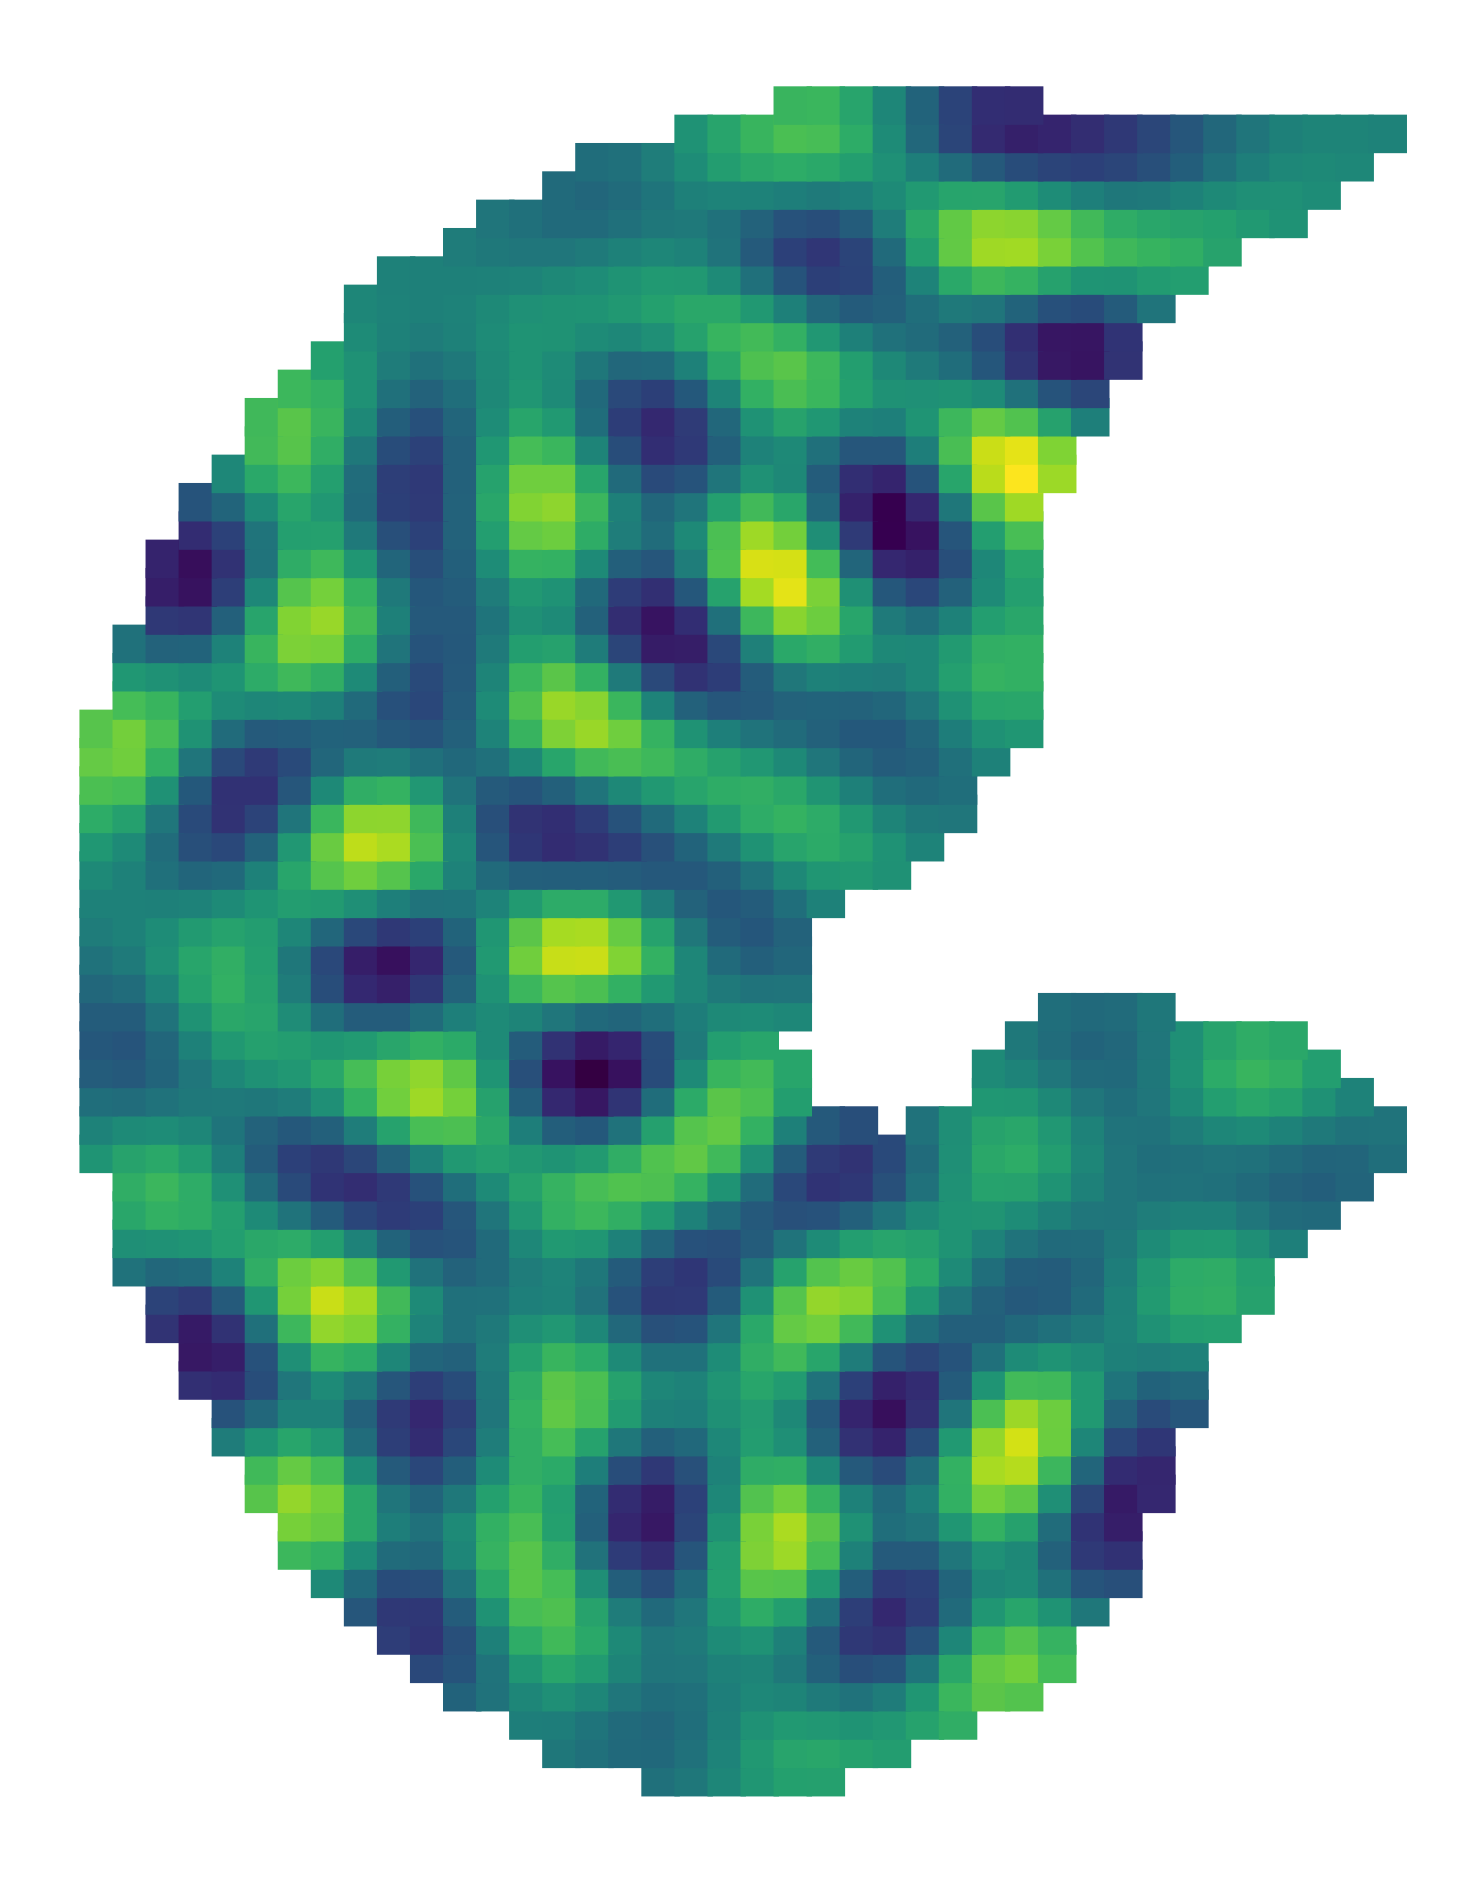
\includegraphics[height=1.5in]{EV100}
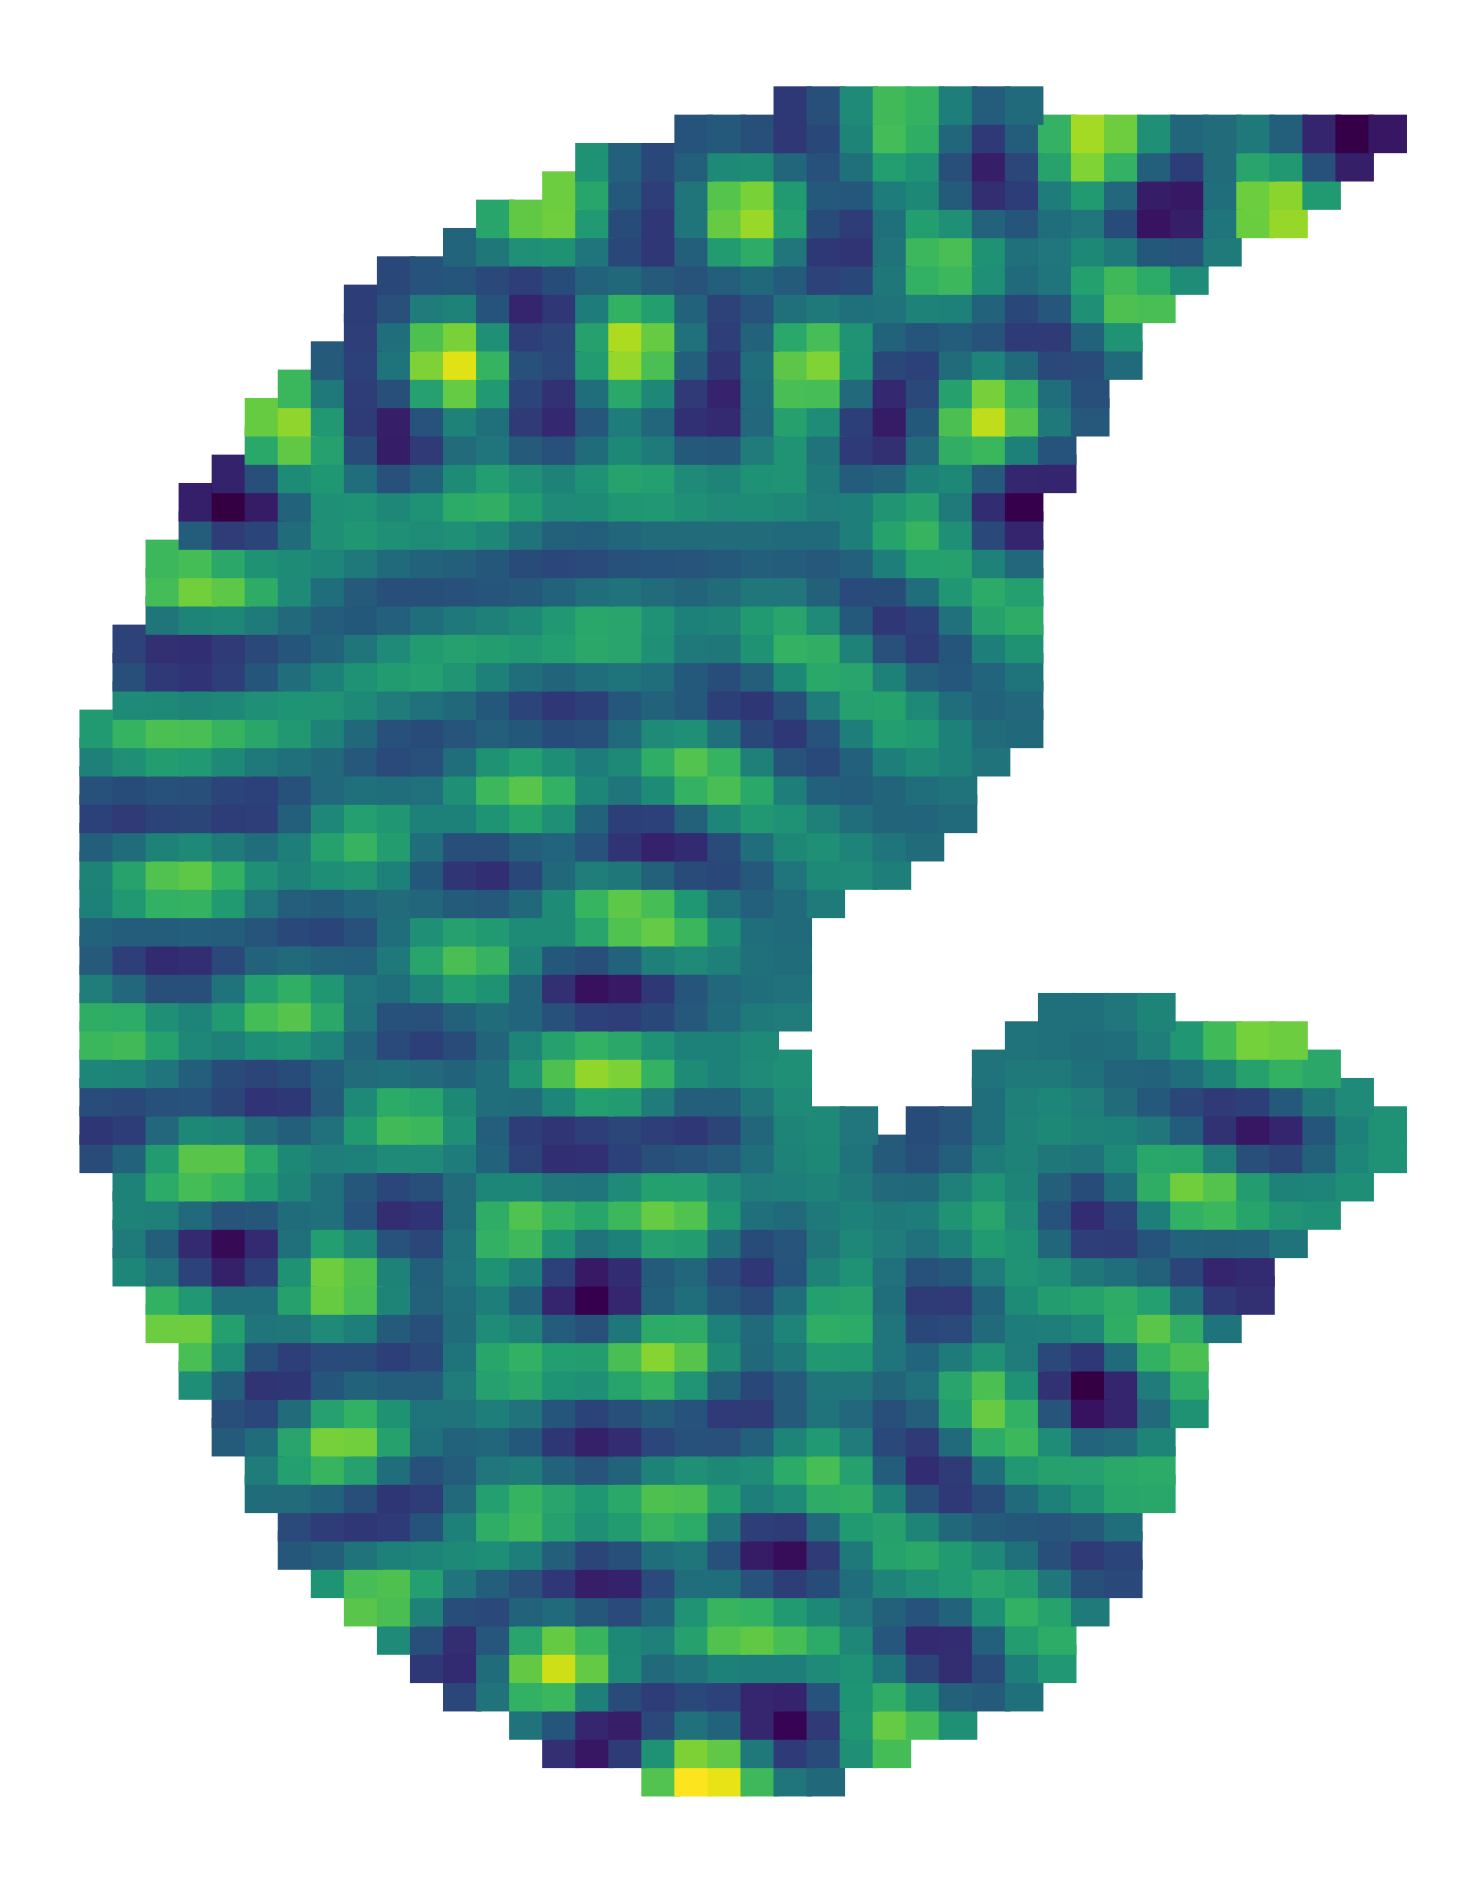
\includegraphics[height=1.5in]{EV200}
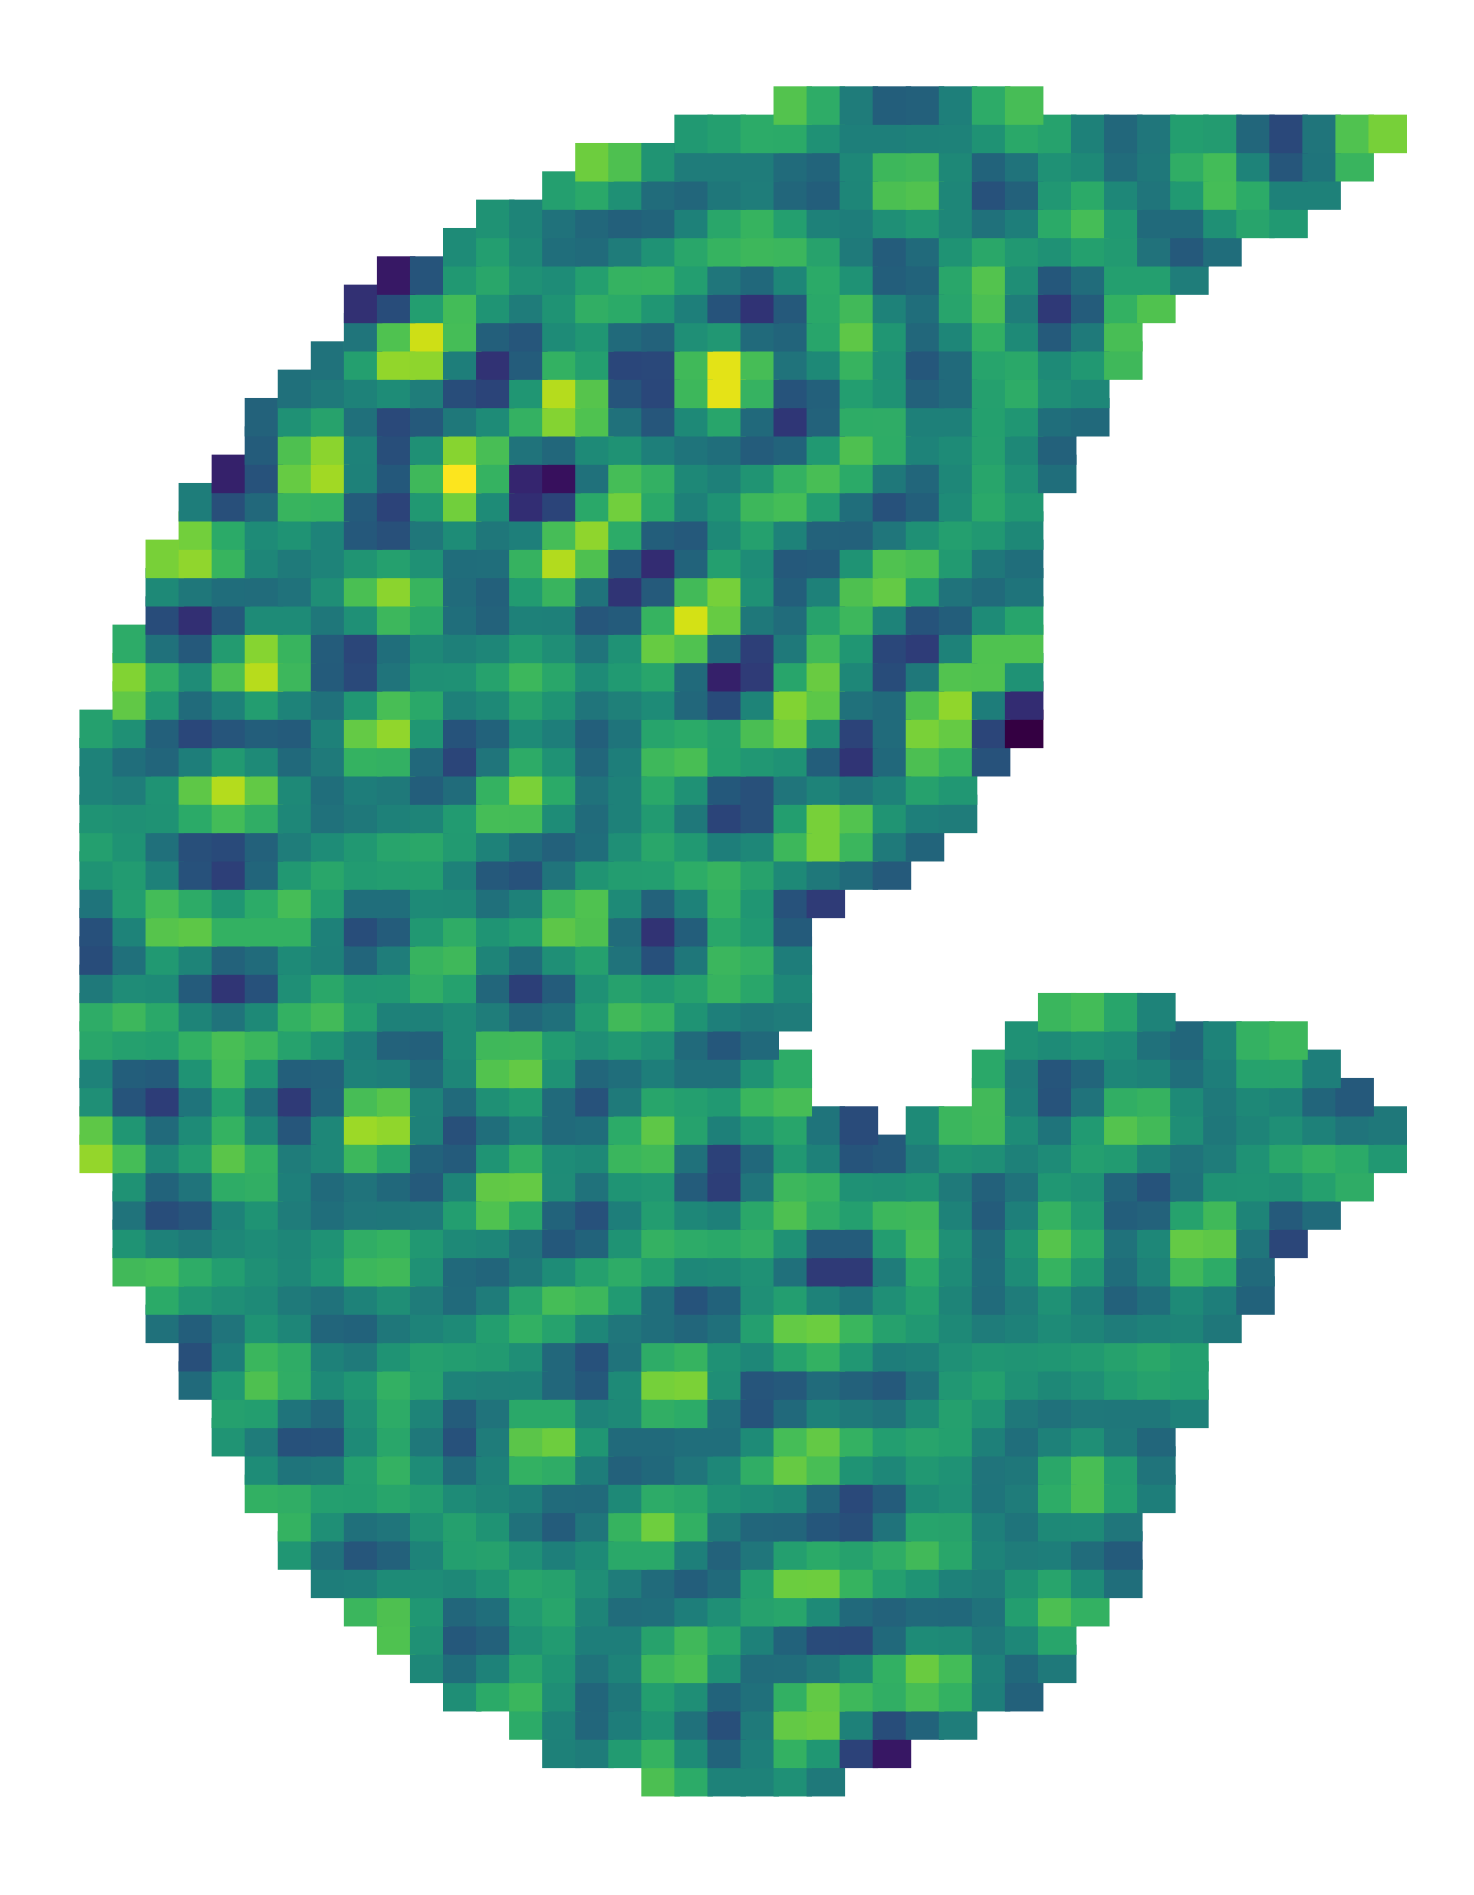
\includegraphics[height=1.5in]{EV300}
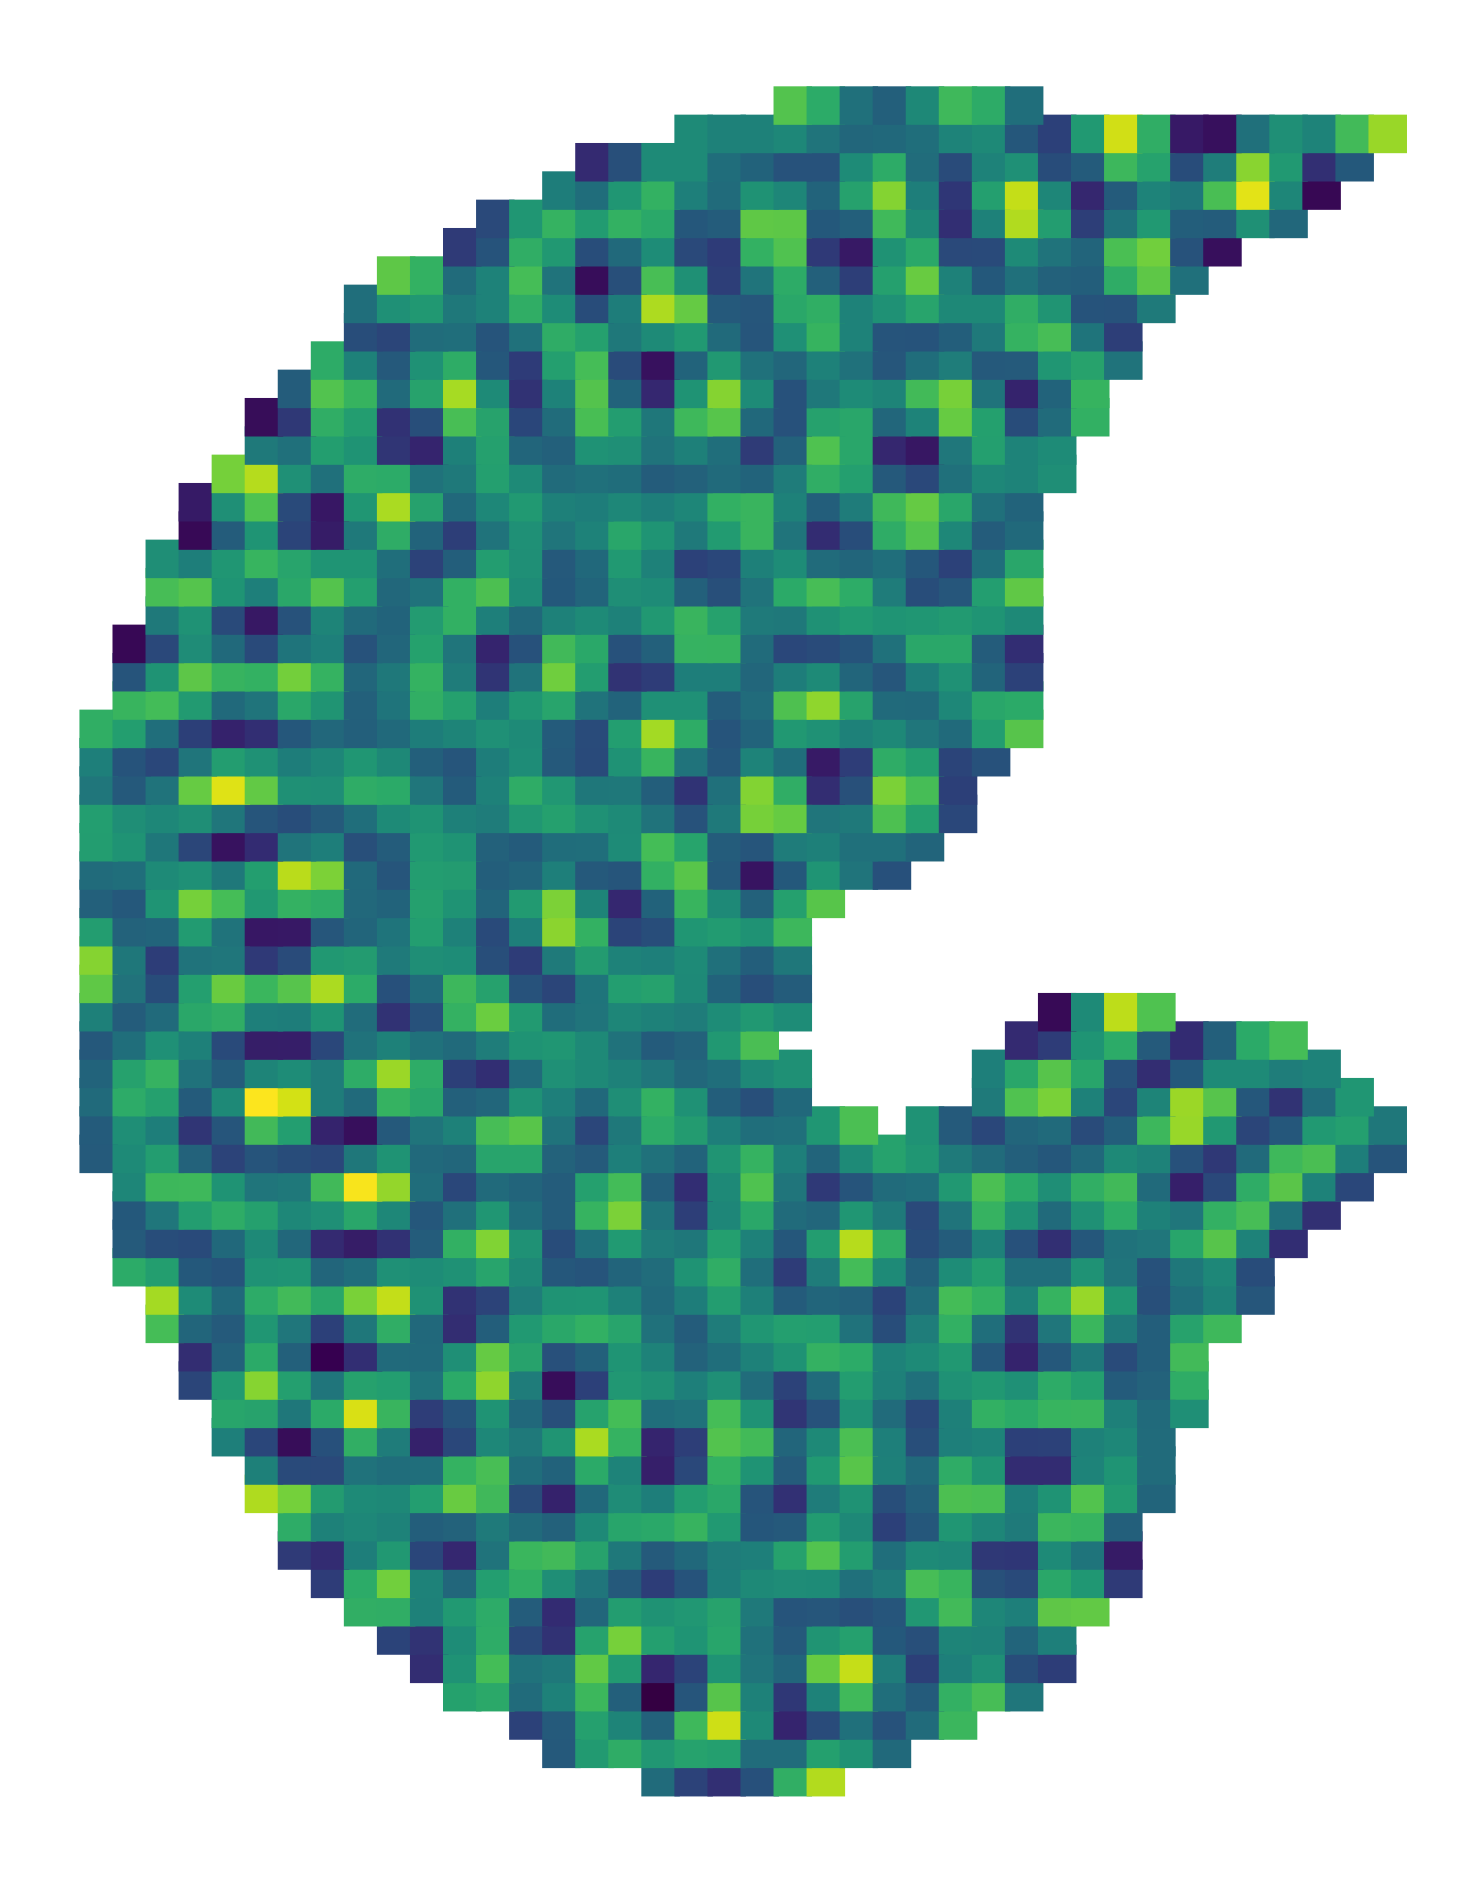
\includegraphics[height=1.5in]{EV397}  
\caption{Moran eigenvectors based on [a specific correlation model for] a template 2D axial slice of the lung. The top row corresponds to the 1st - 4th eigenvectors. The bottom row corresponds to the 100th, 200th, 300th, and 397th eigenvectors. }
\label{fig:eigenvectors}
\end{figure}

\subsubsection{Graph signal processing}

[Siyang, could you try to put in a very rough draft of a GSP section corresponding to the ESF above? It is perfectly okay to mention connections to Fourier theory without recreating the full theory.]

\subsection{Links between the two developments}

\subsection{Simulation}
Yue writing up some ideas for the simulations

\subsection{Application to toy example}
\begin{enumerate}
\item{Fit Sarah's model to the toy example}
\item{Predictive model---need to be reminded of what this is}
\item{Use a GSP framework to build network}
\item{Assume spatial correlation network (weight matrix) for an analysis using GSP--what citation do we want to model}
\end{enumerate}

Investigate using different networks to understand how sensitive results are to the specification of the network.

What are 1-2 other features to investigate.

\begin{enumerate}
\item{Fit Sarah's model to GRADS data}
\item{Predictive model---need to be reminded of what this is}
\item{Use a GSP framework to build network on GRADS data}
\item{Assume spatial correlation network (weight matrix) for an analysis using GSP--what citation do we want to model}
\end{enumerate}

\begin{enumerate}
\item{Fit Sarah's model to BioAD data--need to figure out the subsection to use}
\item{Predictive model---need to be reminded of what this is}
\item{Use a GSP framework to build network on BioAD data}
\item{Assume spatial correlation network (weight matrix) for an analysis using GSP--what citation do we want to model}
\end{enumerate}

\section{Discussion}
We posit(?) that eigendecomposition provides a novel construct for studying factors that influence correlation.

\end{document}

